\section{CycleGAN, Image-to-Image Translation}

In this notebook, we're going to define and train a CycleGAN to read in
an image from a set \(X\) and transform it so that it looks as if it
belongs in set \(Y\). Specifically, we'll look at a set of images of
\href{https://en.wikipedia.org/wiki/Yosemite_National_Park}{Yosemite
national park} taken either during the summer of winter. The seasons are
our two domains!

\begin{quote}
The objective will be to train generators that learn to transform an
image from domain \(X\) into an image that looks like it came from
domain \(Y\) (and vice versa).
\end{quote}

Some examples of image data in both sets are pictured below.

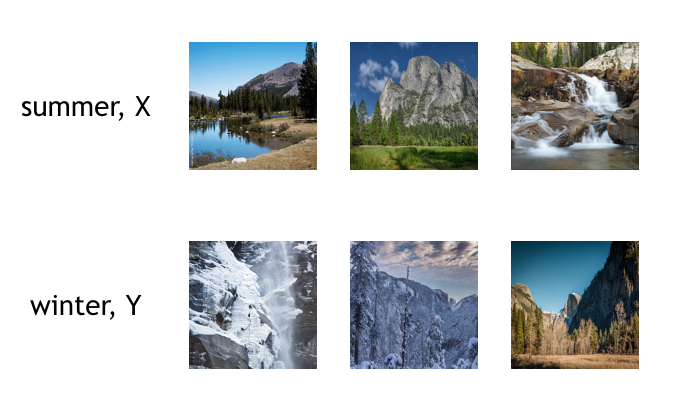
\includegraphics[width=1\linewidth]{img//genAdvNet//image2image/XY_season_images.png}

\subsubsection{Unpaired Training Data}

These images do not come with labels, but CycleGANs give us a way to
learn the mapping between one image domain and another using an
\textbf{unsupervised} approach. A CycleGAN is designed for
image-to-image translation and it learns from unpaired training data.
This means that in order to train a generator to translate images from
domain \(X\) to domain \(Y\), we do not have to have exact
correspondences between individual images in those domains. For example,
in \href{https://arxiv.org/abs/1703.10593}{the paper that introduced
CycleGANs}, the authors are able to translate between images of horses
and zebras, even though there are no images of a zebra in exactly the
same position as a horse or with exactly the same background, etc. Thus,
CycleGANs enable learning a mapping from one domain \(X\) to another
domain \(Y\) without having to find perfectly-matched, training pairs!

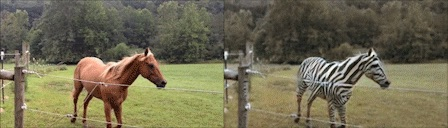
\includegraphics[width=1\linewidth]{img//genAdvNet//image2image/horse2zebra.jpg}

\subsubsection{CycleGAN and Notebook Structure}

A CycleGAN is made of two types of networks: \textbf{discriminators, and
generators}. In this example, the discriminators are responsible for
classifying images as real or fake (for both \(X\) and \(Y\) kinds of
images). The generators are responsible for generating convincing, fake
images for both kinds of images. \newline

This notebook will detail the steps you should take to define and train
such a CycleGAN.

\begin{quote}
\begin{enumerate}
\item You'll load in the image data using PyTorch's DataLoader class to
  efficiently read in images from a specified directory.
\item Then, you'll be tasked with defining the CycleGAN architecture
  according to provided specifications. You'll define the discriminator
  and the generator models.
\item You'll complete the training cycle by calculating the adversarial and
  cycle consistency losses for the generator and discriminator network
  and completing a number of training epochs. \emph{It's suggested that
  you enable GPU usage for training.}
\item Finally, you'll evaluate your model by looking at the loss over time
  and looking at sample, generated images.
\end{enumerate}
\end{quote}

\subsection{Load and Visualize the Data}

We'll first load in and visualize the training data, importing the
necessary libraries to do so.

\begin{lstlisting}[language=Python]
# loading in and transforming data
import os
from typing import Callable

import torch
from torch.utils.data import DataLoader
import torchvision
import torchvision.datasets as datasets
import torchvision.transforms as transforms

# visualizing data
import matplotlib.pyplot as plt
import numpy as np
import warnings

%matplotlib inline
\end{lstlisting}

\subsubsection{DataLoaders}

The \lstinline{get_data_loader} function returns
training and test DataLoaders that can load data efficiently and in
specified batches. The function has the following parameters: 
*
\lstinline{image_type}: \lstinline{summer}
or \lstinline{winter}, the names of the directories where
the X and Y images are stored 
\begin{itemize}
    \item \lstinline{image_dir}: name of the main image directory, which holds all training and test images
    \item \lstinline{image_size}: resized, square image dimension (all images will be resized to this dim)
    \item \lstinline{batch_size}: number of images in one batch of
    \item data
\end{itemize}

The test data is strictly for feeding to our generators, later on, so we
can visualize some generated samples on fixed, test data. \newline

You can see that this function is also responsible for making sure our
images are of the right, square size (128x128x3) and converted into
Tensor image types. \newline

\textbf{It's suggested that you use the default values of these
parameters.}\newline

Note: If you are trying this code on a different set of data, you may
get better results with larger \lstinline{image_size} and
\lstinline{batch_size} parameters. If you change the
\lstinline{batch_size}, make sure that you create
complete batches in the training loop otherwise you may get an error
when trying to save sample data.

\begin{lstlisting}[language=Python]
def get_data_loader(image_type: str, 
                    transform: Callable,
                    image_dir: str = 'summer2winter_yosemite', 
                    batch_size: int = 16, 
                    num_workers: int = 0):
    """Returns training and test data loaders for a given image type, either 'summer' or 'winter'. 
       These images will be resized to 128x128x3, by default, converted into Tensors, and normalized.
    """
    
    # get training and test directories
    image_path = image_dir
    train_path = os.path.join(image_path, image_type)
    test_path = os.path.join(image_path, 'test_{}'.format(image_type))

    # define datasets using ImageFolder
    train_dataset = datasets.ImageFolder(train_path, transform)
    test_dataset = datasets.ImageFolder(test_path, transform)

    # create and return DataLoaders
    train_loader = DataLoader(dataset=train_dataset, batch_size=batch_size, shuffle=True, num_workers=num_workers)
    test_loader = DataLoader(dataset=test_dataset, batch_size=batch_size, shuffle=False, num_workers=num_workers)

    return train_loader, test_loader
\end{lstlisting}

\begin{lstlisting}[language=Python]
from torchvision.transforms import Compose, Resize, ToTensor, Normalize 
\end{lstlisting}

\begin{lstlisting}[language=Python]
# Create train and test dataloaders for images from the two domains X and Y
# image_type = directory names for our data
# resize and normalize the images
image_size = 128
transform = Compose([Resize(image_size), # resize to 128x128
                     ToTensor(),
                     Normalize([0.5, 0.5, 0.5], [0.5, 0.5, 0.5])])
    
dataloader_X, test_dataloader_X = get_data_loader(image_type='summer', 
                                                  transform=transform,
                                                  image_dir='../summer2winter_yosemite/',)
dataloader_Y, test_dataloader_Y = get_data_loader(image_type='winter', 
                                                  transform=transform,
                                                  image_dir='../summer2winter_yosemite/',)
\end{lstlisting}

\subsection{Display some Training Images}

Below we provide a function \lstinline{imshow} that
reshape some given images and converts them to NumPy images so that they
can be displayed by \lstinline{plt}. This cell should
display a grid that contains a batch of image data from set \(X\).

\begin{lstlisting}[language=Python]
# helper imshow function
def imshow(img):
    npimg = img.numpy()
    npimg = (((npimg + 1) * 255) / 2).astype(np.uint8)
    plt.imshow(np.transpose(npimg, (1, 2, 0)))
    

# get some images from X
dataiter = iter(dataloader_X)
# the "_" is a placeholder for no labels
images, _ = dataiter.next()

# show images
fig = plt.figure(figsize=(12, 8))
imshow(torchvision.utils.make_grid(images))
\end{lstlisting}

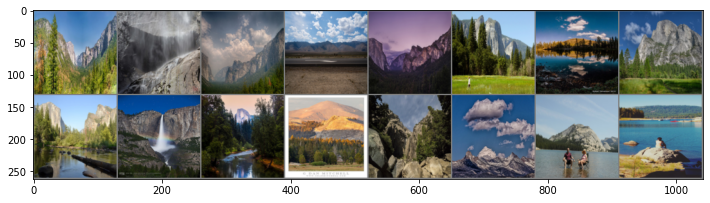
\includegraphics{img//genAdvNet//image2image/output_8_0.png}

Next, let's visualize a batch of images from set \(Y\).

\begin{lstlisting}[language=Python]
# get some images from Y
dataiter = iter(dataloader_Y)
images, _ = dataiter.next()

# show images
fig = plt.figure(figsize=(12,8))
imshow(torchvision.utils.make_grid(images))
\end{lstlisting}

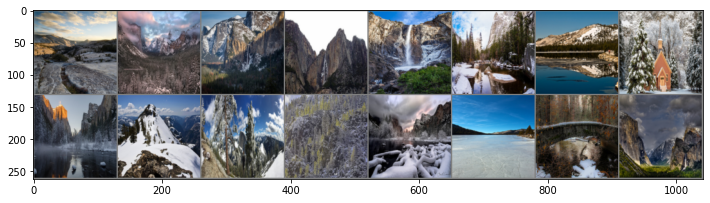
\includegraphics{img//genAdvNet//image2image/output_10_0.png}

\subsection{Define the Model}

A CycleGAN is made of two discriminator and two generator networks.

\subsection{Discriminators}

The discriminators, \(D_X\) and \(D_Y\), in this CycleGAN are
convolutional neural networks that see an image and attempt to classify
it as real or fake. In this case, real is indicated by an output close
to 1 and fake as close to 0. The discriminators have the following
architecture:

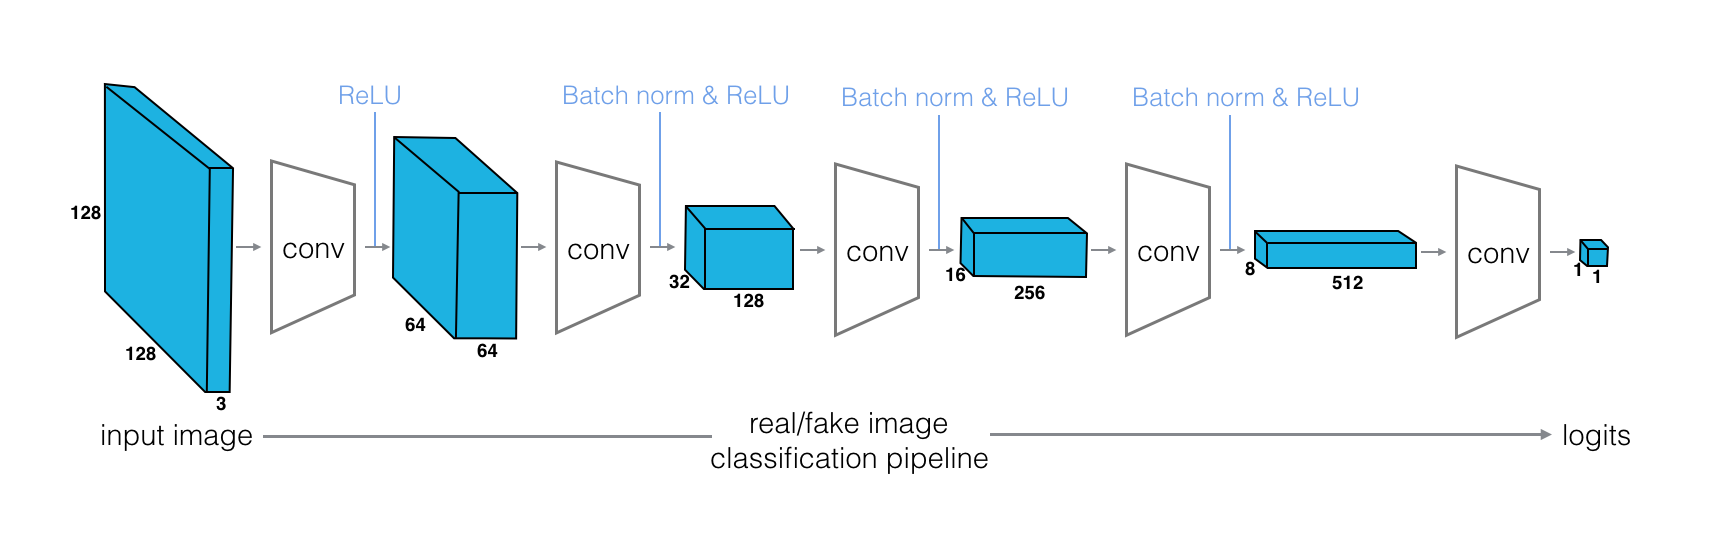
\includegraphics[width=1\linewidth]{img//genAdvNet//image2image/discriminator_layers.png}

This network sees a 128x128x3 image, and passes it through 5
convolutional layers that downsample the image by a factor of 2. The
first four convolutional layers have a BatchNorm and ReLu activation
function applied to their output, and the last acts as a classification
layer that outputs one value.

\subsubsection{Convolutional Helper Function}

To define the discriminators, you're expected to use the provided
\lstinline{conv} function, which creates a convolutional
layer + an optional batch norm layer.

\begin{lstlisting}[language=Python]
import torch.nn as nn
\end{lstlisting}

\begin{lstlisting}[language=Python]
class ConvBlock(nn.Module):
    """
    A convolutional block is made of 3 layers: Conv -> BatchNorm -> Activation.
    args:
    - in_channels: number of channels in the input to the conv layer
    - out_channels: number of filters in the conv layer
    - kernel_size: filter dimension of the conv layer
    - stride: stride of the conv layer
    - use_bn: whether to use batch normalization or not
    - use_activation: whether to use an activation function or not
    """
    def __init__(self, 
                 in_channels: int, 
                 out_channels: int, 
                 kernel_size: int,
                 stride: int = 1,
                 padding: int = 1,
                 use_bn: bool = True,
                 use_activation: bool = True):
        super(ConvBlock, self).__init__()
        
        self.conv = nn.Conv2d(in_channels, out_channels, kernel_size, stride=stride, padding=padding, bias=False)
        
        self.use_bn = use_bn
        if self.use_bn:
            self.bn = nn.BatchNorm2d(out_channels)
            
        self.use_activation = use_activation
        if self.use_activation:
            self.act = nn.ReLU()
        
    def forward(self, x: torch.Tensor) -> torch.Tensor:
        x = self.conv(x)
        if self.use_bn:
            x = self.bn(x)
        if self.use_activation:
            x = self.act(x)
        return x
\end{lstlisting}

\subsubsection{Define the Discriminator Architecture}

Your task is to fill in the \lstinline{__init__}
function with the specified 5 layer conv net architecture. Both \(D_X\)
and \(D_Y\) have the same architecture, so we only need to define one
class, and later instantiate two discriminators. \textgreater{} It's
recommended that you use a \textbf{kernel size of 4x4} and use that to
determine the correct stride and padding size for each layer.
\href{http://cs231n.github.io/convolutional-networks/\#conv}{This
Stanford resource} may also help in determining stride and padding
sizes.

\begin{itemize}

\item  Define your convolutional layers in \lstinline{__init__}
\item  Then fill in the forward behavior of the network
\end{itemize}

The \lstinline{forward} function defines how an input
image moves through the discriminator, and the most important thing is
to pass it through your convolutional layers in order, with a
\textbf{ReLu} activation function applied to all but the last layer.\newline

You should \textbf{not} apply a sigmoid activation function to the
output, here, and that is because we are planning on using a squared
error loss for training. And you can read more about this loss function,
later in the notebook.

\begin{lstlisting}[language=Python]
class Discriminator(nn.Module):
    
    def __init__(self, conv_dim=64):
        super(Discriminator, self).__init__()

        # Define all convolutional layers
        # Should accept an RGB image as input and output a single value

        # Convolutional layers, increasing in depth
        # first layer has *no* batchnorm
        self.conv1 = ConvBlock(3, conv_dim, 4, stride=2, use_bn=False) # x, y = 64, depth 64
        self.conv2 = ConvBlock(conv_dim, conv_dim*2, 4, stride=2, ) # (32, 32, 128)
        self.conv3 = ConvBlock(conv_dim*2, conv_dim*4, 4, stride=2) # (16, 16, 256)
        self.conv4 = ConvBlock(conv_dim*4, conv_dim*8, 4, stride=2) # (8, 8, 512)
        # Classification layer
        self.conv5 = ConvBlock(conv_dim*8, 1, 8, stride=1, padding=0, use_bn=False, use_activation=False)
        

    def forward(self, x):
        # relu applied to all conv layers but last
        out = self.conv1(x)
        out = self.conv2(out)
        out = self.conv3(out)
        out = self.conv4(out)
        # last, classification layer
        out = self.conv5(out)
        return out
\end{lstlisting}

\subsection{Generators}

The generators, \lstinline{G_XtoY} and
\lstinline{G_YtoX} (sometimes called F), are made of an
\textbf{encoder}, a conv net that is responsible for turning an image
into a smaller feature representation, and a \textbf{decoder}, a
\emph{transpose\_conv} net that is responsible for turning that
representation into an transformed image. These generators, one from
XtoY and one from YtoX, have the following architecture:

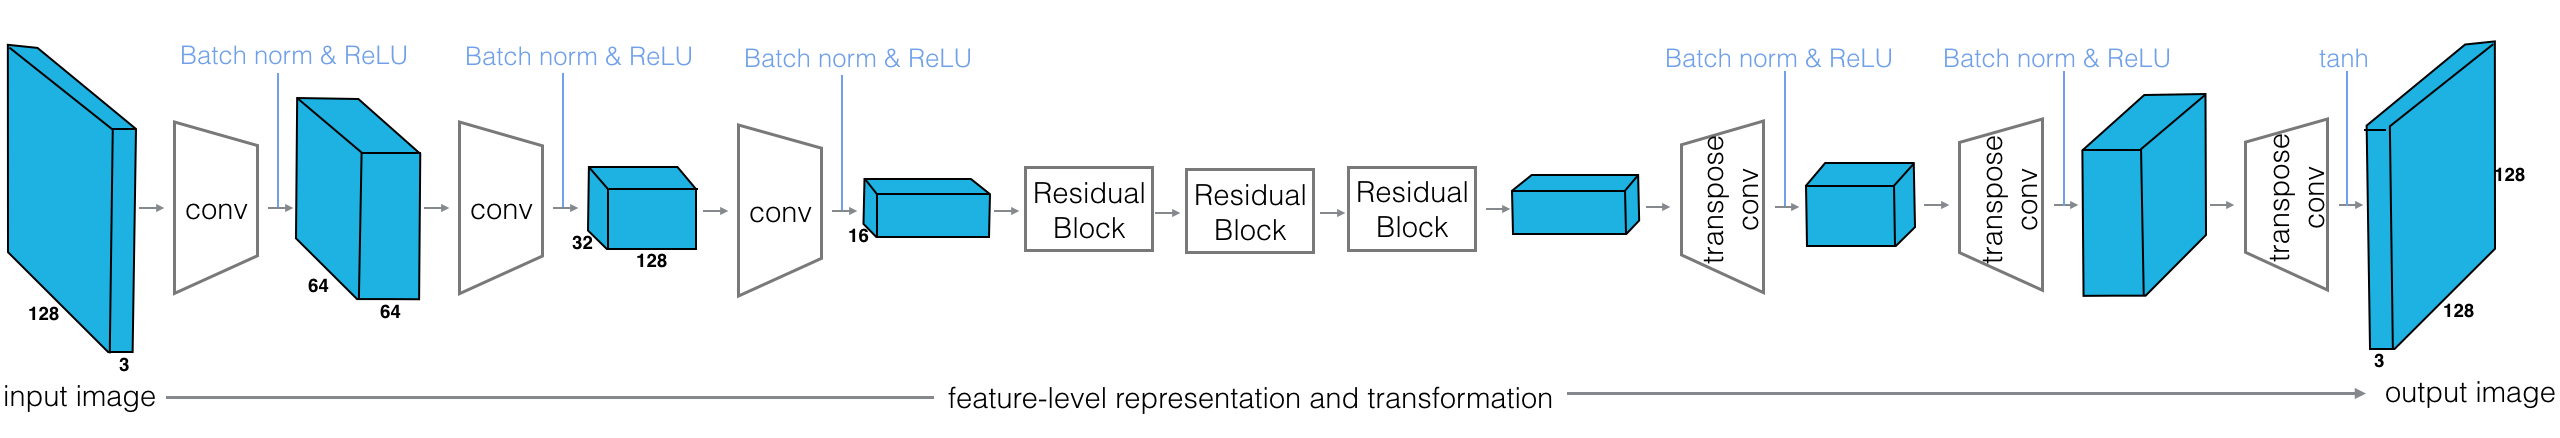
\includegraphics[width=1\linewidth]{img//genAdvNet//image2image/cyclegan_generator_ex.png}

This network sees a 128x128x3 image, compresses it into a feature
representation as it goes through three convolutional layers and reaches
a series of residual blocks. It goes through a few (typically 6 or more)
of these residual blocks, then it goes through three transpose
convolutional layers (sometimes called \emph{de-conv} layers) which
upsample the output of the resnet blocks and create a new image!\newline

Note that most of the convolutional and transpose-convolutional layers
have BatchNorm and ReLu functions applied to their outputs with the
exception of the final transpose convolutional layer, which has a
\lstinline{tanh} activation function applied to the
output. Also, the residual blocks are made of convolutional and batch
normalization layers, which we'll go over in more detail, next.

\subsubsection{Residual Block Class}

To define the generators, you're expected to define a
\lstinline{ResidualBlock} class which will help you
connect the encoder and decoder portions of the generators. You might be
wondering, what exactly is a Resnet block? It may sound familiar from
something like ResNet50 for image classification, pictured below.

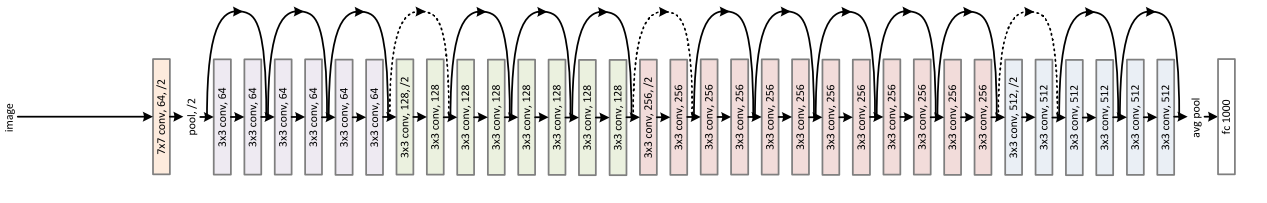
\includegraphics[width=1\linewidth]{img//genAdvNet//image2image/resnet_50.png}

ResNet blocks rely on connecting the output of one layer with the input
of an earlier layer. The motivation for this structure is as follows:
very deep neural networks can be difficult to train. Deeper networks are
more likely to have vanishing or exploding gradients and, therefore,
have trouble reaching convergence; batch normalization helps with this a
bit. However, during training, we often see that deep networks respond
with a kind of training degradation. Essentially, the training accuracy
stops improving and gets saturated at some point during training. In the
worst cases, deep models would see their training accuracy actually
worsen over time!\newline

One solution to this problem is to use \textbf{Resnet blocks} that allow
us to learn so-called \emph{residual functions} as they are applied to
layer inputs. You can read more about this proposed architecture in the
paper, \href{https://arxiv.org/pdf/1512.03385.pdf}{Deep Residual
Learning for Image Recognition} by Kaiming He et. al, and the below
image is from that paper.

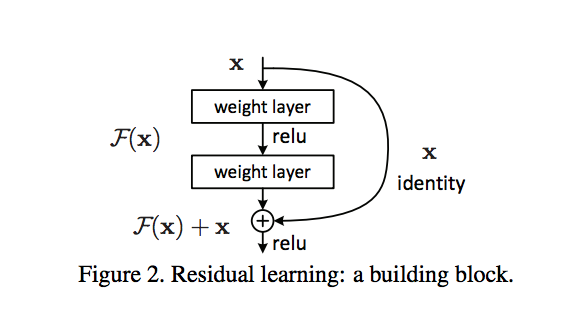
\includegraphics[width=0.5\linewidth]{img//genAdvNet//image2image/resnet_block.png}

\subsubsection{Residual Functions}

Usually, when we create a deep learning model, the model (several layers
with activations applied) is responsible for learning a mapping,
\lstinline{M}, from an input \lstinline{x}
to an output \lstinline{y}.
\textgreater{}\lstinline{M(x) = y} (Equation 1) \newline

Instead of learning a direct mapping from \lstinline{x} to
\lstinline{y}, we can instead define a \textbf{residual function} \lstinline{F(x) = M(x) - x} \newline

This looks at the difference between a mapping applied to x and the
original input, x. \lstinline{F(x)} is, typically, two
convolutional layers + normalization layer and a ReLu in between. These
convolutional layers should have the same number of inputs as outputs.
This mapping can then be written as the following; a function of the
residual function and the input x. The addition step creates a kind of
loop that connects the input x to the output, y:
\textgreater{}\lstinline{M(x) = F(x) + x} (Equation 2) or

\begin{quote}
\lstinline{y = F(x) + x} (Equation 3)
\end{quote}

\paragraph{Optimizing a Residual Function}

The idea is that it is easier to optimize this residual function
\lstinline{F(x)} than it is to optimize the original
mapping \lstinline{M(x)}. Consider an example; what if we
want \lstinline{y = x}? \newline

From our first, direct mapping equation, \textbf{Equation 1}, we could
set \lstinline{M(x) = x} but it is easier to solve the
residual equation \lstinline{F(x) = 0}, which, when
plugged in to \textbf{Equation 3}, yields
\lstinline{y = x}.

\subsubsection{\texorpdfstring{Defining the \texttt{ResidualBlock} Class}{Defining the ResidualBlock Class}}

To define the \lstinline{ResidualBlock} class, we'll
define residual functions (a series of layers), apply them to an input x
and add them to that same input. This is defined just like any other
neural network, with an \lstinline{__init__} function
and the addition step in the \lstinline{forward} function. \newline

In our case, you'll want to define the residual block as: 
\begin{itemize}
    \item Two convolutional layers with the same size input and output
    \item Batch normalization applied to the outputs of the convolutional layers
    \item A ReLu function on the output of the \emph{first} convolutional layer
\end{itemize}

Then, in the \lstinline{forward} function, add the input x
to this residual block. Feel free to use the helper
\lstinline{conv} function from above to create this block.

\begin{lstlisting}[language=Python]
# residual block class
class ResidualBlock(nn.Module):
    """Defines a residual block.
       This adds an input x to a convolutional layer (applied to x) with the same size input and output.
       These blocks allow a model to learn an effective transformation from one domain to another.
    """
    def __init__(self, conv_dim):
        super(ResidualBlock, self).__init__()
        # conv_dim = number of inputs
        # define two convolutional layers + batch normalization that will act as our residual function, F(x)
        # layers should have the same shape input as output; I suggest a kernel_size of 3
        self.conv_block1 = ConvBlock(in_channels=conv_dim, out_channels=conv_dim, kernel_size=3)
        self.conv_block2 = ConvBlock(in_channels=conv_dim, out_channels=conv_dim, kernel_size=3, use_activation=False)
        
    def forward(self, x):
        # apply a ReLu activation the outputs of the first layer
        # return a summed output, x + resnet_block(x)
        out_1 = self.conv_block1(x)
        out_2 = x + self.conv_block2(out_1)
        return out_2
\end{lstlisting}

\subsubsection{Transpose Convolutional Helper Function}

To define the generators, you're expected to use the above
\lstinline{conv} function,
\lstinline{ResidualBlock} class, and the below
\lstinline{deconv} helper function, which creates a
transpose convolutional layer + an optional batchnorm layer.

\begin{lstlisting}[language=Python]
class DeconvBlock(nn.Module):
    """
    A "de-convolutional" block is made of 3 layers: ConvTranspose -> BatchNorm -> Activation.
    args:
    - in_channels: number of channels in the input to the conv layer
    - out_channels: number of filters in the conv layer
    - kernel_size: filter dimension of the conv layer
    - stride: stride of the conv layer
    - padding: padding of the conv layer
    - batch_norm: whether to use batch norm or not
    """
    def __init__(self, 
                 in_channels: int, 
                 out_channels: int, 
                 kernel_size: int, 
                 stride: int = 2,
                 padding: int = 1,
                 batch_norm: bool = True):
        super(DeconvBlock, self).__init__()
        self.deconv = nn.ConvTranspose2d(in_channels, out_channels, kernel_size, stride, padding, bias=False)
        self.batch_norm = batch_norm
        if self.batch_norm:
            self.bn = nn.BatchNorm2d(out_channels)
        self.activation = nn.ReLU()
        
    def forward(self, x: torch.Tensor) -> torch.Tensor:
        x = self.deconv(x)
        if self.batch_norm:
            x = self.bn(x)
        x = self.activation(x)
        return x
\end{lstlisting}

\subsection{Define the Generator Architecture}

\begin{itemize}
\item Complete the \lstinline{__init__} function with the
  specified 3 layer \textbf{encoder} convolutional net, a series of
  residual blocks (the number of which is given by
  \lstinline{n_res_blocks}), and then a 3 layer
  \textbf{decoder} transpose convolutional net.
\item Then complete the \lstinline{forward} function to define
  the forward behavior of the generators. Recall that the last layer has
  a \lstinline{tanh} activation function.
\end{itemize}

Both \(G_{XtoY}\) and \(G_{YtoX}\) have the same architecture, so we
only need to define one class, and later instantiate two generators.
\begin{lstlisting}[language=Python]
class CycleGenerator(nn.Module):
    
    def __init__(self, conv_dim: int = 64, n_res_blocks: int = 6):
        super(CycleGenerator, self).__init__()

        # 1. Define the encoder part of the generator
        
        # initial convolutional layer given, below
        self.conv1 = ConvBlock(3, conv_dim, 4, stride=2)
        self.conv2 = ConvBlock(conv_dim, conv_dim*2, 4, stride=2)
        self.conv3 = ConvBlock(conv_dim*2, conv_dim*4, 4, stride=2)

        # 2. Define the resnet part of the generator
        # Residual blocks
        self.res_layers = nn.ModuleList()
        for layer in range(n_res_blocks):
            self.res_layers.append(ResidualBlock(conv_dim*4))

        # 3. Define the decoder part of the generator
        # two transpose convolutional layers and a third that looks a lot like the initial conv layer
        self.deconv1 = DeconvBlock(conv_dim*4, conv_dim*2, 4)
        self.deconv2 = DeconvBlock(conv_dim*2, conv_dim, 4)
        # no batch norm on last layer
        self.deconv3 = nn.ConvTranspose2d(conv_dim, 3, 4, 2, 1, bias=False)
        
        self.final_act = nn.Tanh()
        
    def forward(self, x: torch.Tensor) -> torch.Tensor:
        """Given an image x, returns a transformed image."""
        # define feedforward behavior, applying activations as necessary
        out = self.conv1(x)
        out = self.conv2(out)
        out = self.conv3(out)
        
        for layer in self.res_layers:
            out = layer(out)
        
        out = self.deconv1(out)
        out = self.deconv2(out)
        # tanh applied to last layer
        out = self.deconv3(out)
        out = self.final_act(out)
        return out
\end{lstlisting}

\subsection{Create the complete network}

Using the classes you defined earlier, you can define the discriminators
and generators necessary to create a complete CycleGAN. The given
parameters should work for training.\newline

First, create two discriminators, one for checking if \(X\) sample
images are real, and one for checking if \(Y\) sample images are real.
Then the generators. Instantiate two of them, one for transforming a
painting into a realistic photo and one for transforming a photo into
into a painting.

\begin{lstlisting}[language=Python]
def create_model(g_conv_dim=64, d_conv_dim=64, n_res_blocks=6):
    """Builds the generators and discriminators."""
    
    # Instantiate generators
    G_XtoY = CycleGenerator(conv_dim=g_conv_dim, n_res_blocks=n_res_blocks)
    G_YtoX = CycleGenerator(conv_dim=g_conv_dim, n_res_blocks=n_res_blocks)
    # Instantiate discriminators
    D_X = Discriminator(conv_dim=d_conv_dim)
    D_Y = Discriminator(conv_dim=d_conv_dim)

    # move models to GPU, if available
    if torch.cuda.is_available():
        device = torch.device("cuda:0")
        G_XtoY.to(device)
        G_YtoX.to(device)
        D_X.to(device)
        D_Y.to(device)
        print('Models moved to GPU.')
    else:
        print('Only CPU available.')

    return G_XtoY, G_YtoX, D_X, D_Y
\end{lstlisting}

\begin{lstlisting}[language=Python]
# call the function to get models
G_XtoY, G_YtoX, D_X, D_Y = create_model()
\end{lstlisting}

\begin{lstlisting}
Only CPU available.
\end{lstlisting}

\subsection{Check that you've implemented this correctly}

The function \lstinline{create_model} should return the
two generator and two discriminator networks. After you've defined these
discriminator and generator components, it's good practice to check your
work. The easiest way to do this is to print out your model architecture
and read through it to make sure the parameters are what you expected.
The next cell will print out their architectures.

\begin{lstlisting}[language=Python]
# helper function for printing the model architecture
def print_models(G_XtoY, G_YtoX, D_X, D_Y):
    """Prints model information for the generators and discriminators.
    """
    print("                     G_XtoY                    ")
    print("-----------------------------------------------")
    print(G_XtoY)
    print()

    print("                     G_YtoX                    ")
    print("-----------------------------------------------")
    print(G_YtoX)
    print()

    print("                      D_X                      ")
    print("-----------------------------------------------")
    print(D_X)
    print()

    print("                      D_Y                      ")
    print("-----------------------------------------------")
    print(D_Y)
    print()
    

# print all of the models
print_models(G_XtoY, G_YtoX, D_X, D_Y)
\end{lstlisting}

\subsection{Discriminator and Generator Losses}

Computing the discriminator and the generator losses are key to getting
a CycleGAN to train.

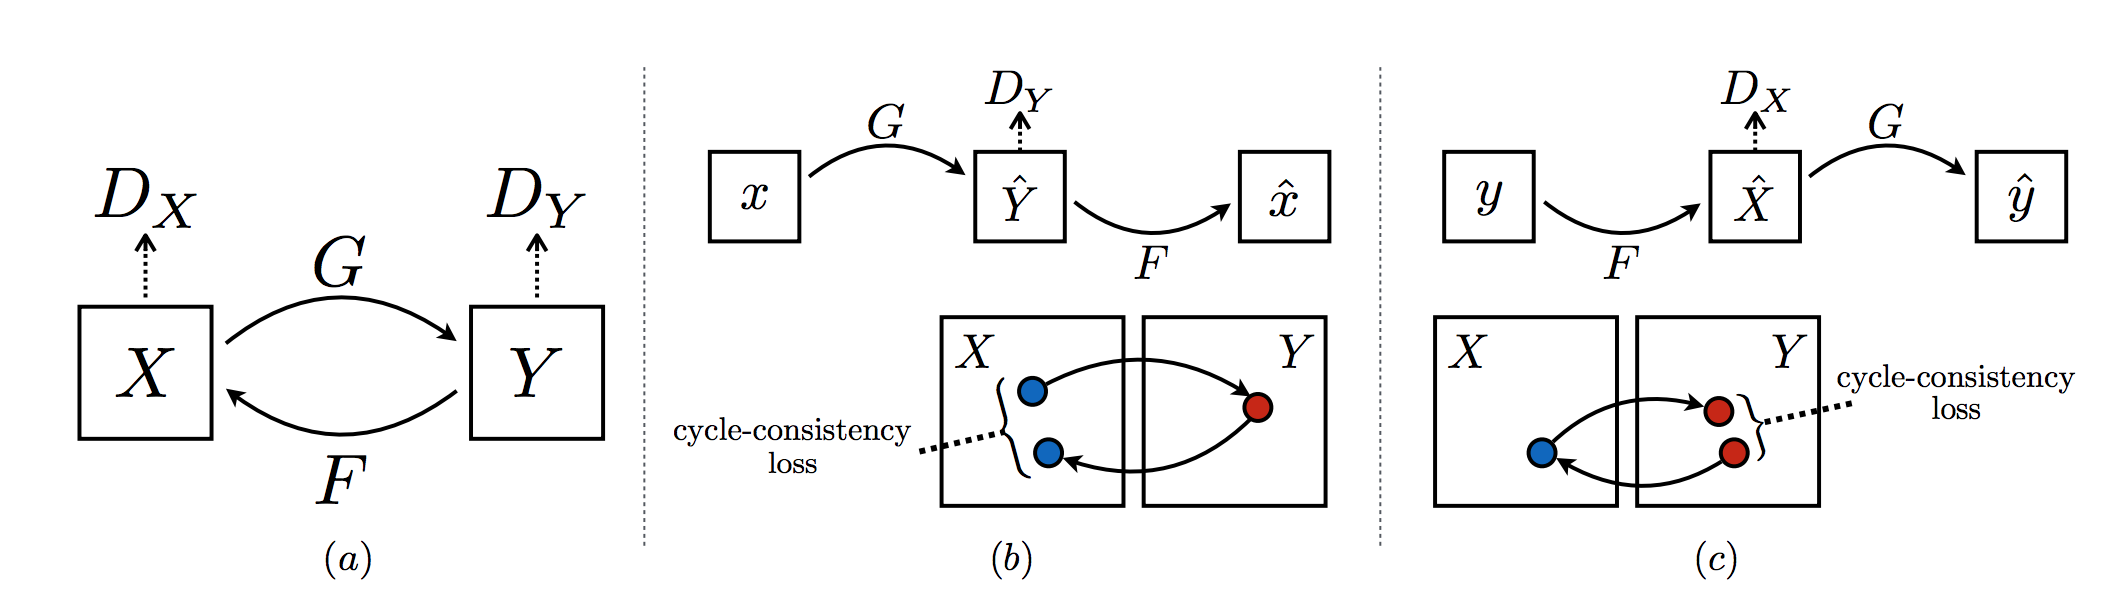
\includegraphics[width=1\linewidth]{img//genAdvNet//image2image/CycleGAN_loss.png}
\captionof{figure}{\textbf{Image from \href{https://arxiv.org/abs/1703.10593}{original paper} by Jun-Yan Zhu et. al.}}

\begin{itemize}
\item The CycleGAN contains two mapping functions \(G: X \rightarrow Y\) and
  \(F: Y \rightarrow X\), and associated adversarial discriminators
  \(D_Y\) and \(D_X\). \textbf{(a)} \(D_Y\) encourages \(G\) to
  translate \(X\) into outputs indistinguishable from domain \(Y\), and
  vice versa for \(D_X\) and \(F\).
\item To further regularize the mappings, we introduce two cycle consistency
  losses that capture the intuition that if we translate from one domain
  to the other and back again we should arrive at where we started.
  \textbf{(b)} Forward cycle-consistency loss and \textbf{(c)} backward
  cycle-consistency loss.
\end{itemize}

\subsection{Least Squares GANs}

We've seen that regular GANs treat the discriminator as a classifier
with the sigmoid cross entropy loss function. However, this loss
function may lead to the vanishing gradients problem during the learning
process. To overcome such a problem, we'll use a least squares loss
function for the discriminator. This structure is also referred to as a
least squares GAN or LSGAN, and you can
\href{https://arxiv.org/pdf/1611.04076.pdf}{read the original paper on
LSGANs, here}. The authors show that LSGANs are able to generate higher
quality images than regular GANs and that this loss type is a bit more
stable during training!

\subsubsection{Discriminator Losses}

The discriminator losses will be mean squared errors between the output
of the discriminator, given an image, and the target value, 0 or 1,
depending on whether it should classify that image as fake or real. For
example, for a \emph{real} image, \lstinline{x}, we can
train \(D_X\) by looking at how close it is to recognizing and image
\lstinline{x} as real using the mean squared error:

\begin{lstlisting}
out_x = D_X(x)
real_err = torch.mean((out_x-1)**2)
\end{lstlisting}

\subsubsection{Generator Losses}

Calculating the generator losses will look somewhat similar to
calculating the discriminator loss; there will still be steps in which
you generate fake images that look like they belong to the set of \(X\)
images but are based on real images in set \(Y\), and vice versa. You'll
compute the ``real loss'' on those generated images by looking at the
output of the discriminator as it's applied to these \emph{fake} images;
this time, your generator aims to make the discriminator classify these
fake images as \emph{real} images.

\paragraph{Cycle Consistency Loss}

In addition to the adversarial losses, the generator loss terms will
also include the \textbf{cycle consistency loss}. This loss is a measure
of how good a reconstructed image is, when compared to an original
image. \newline

Say you have a fake, generated image, \lstinline{x_hat},
and a real image, \lstinline{y}. You can get a
reconstructed \lstinline{y_hat} by applying
\lstinline{G_XtoY(x_hat) = y_hat} and then check to see
if this reconstruction \lstinline{y_hat} and the orginal
image \lstinline{y} match. For this, we recommed
calculating the L1 loss, which is an absolute difference, between
reconstructed and real images. You may also choose to multiply this loss
by some weight value \lstinline{lambda_weight} to convey
its importance.

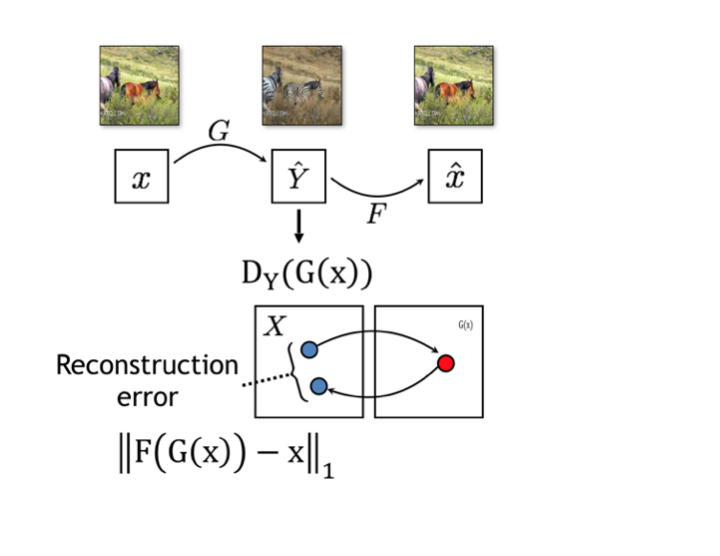
\includegraphics[width=1\linewidth]{img//genAdvNet//image2image/reconstruction_error.png}

The total generator loss will be the sum of the generator losses and the
forward and backward cycle consistency losses.

\subsubsection{Define Loss Functions}

To help us calculate the discriminator and gnerator losses during
training, let's define some helpful loss functions. Here, we'll define
three. 1. \lstinline{real_mse_loss} that looks at the
output of a discriminator and returns the error based on how close that
output is to being classified as real. This should be a mean squared
error. 2. \lstinline{fake_mse_loss} that looks at the
output of a discriminator and returns the error based on how close that
output is to being classified as fake. This should be a mean squared
error. 3. \lstinline{cycle_consistency_loss} that looks
at a set of real image and a set of reconstructed/generated images, and
returns the mean absolute error between them. This has a
\lstinline{lambda_weight} parameter that will weight the
mean absolute error in a batch.\newline

It's recommended that you take a
\href{https://arxiv.org/pdf/1703.10593.pdf}{look at the original,
CycleGAN paper} to get a starting value for
\lstinline{lambda_weight}.

\begin{lstlisting}[language=Python]
def real_mse_loss(D_out):
    # how close is the produced output from being "real"?
    return torch.mean((D_out-1)**2)

def fake_mse_loss(D_out):
    # how close is the produced output from being "false"?
    return torch.mean(D_out**2)

def cycle_consistency_loss(real_im, reconstructed_im, lambda_weight):
    # calculate reconstruction loss 
    # as absolute value difference between the real and reconstructed images
    reconstr_loss = torch.mean(torch.abs(real_im - reconstructed_im))
    # return weighted loss
    return lambda_weight*reconstr_loss    
\end{lstlisting}

\subsubsection{Define the Optimizers}

Next, let's define how this model will update its weights. This, like
the GANs you may have seen before, uses
\href{https://pytorch.org/docs/stable/optim.html\#algorithms}{Adam}
optimizers for the discriminator and generator. It's again recommended
that you take a \href{https://arxiv.org/pdf/1703.10593.pdf}{look at the
original, CycleGAN paper} to get starting hyperparameter values.

\begin{lstlisting}[language=Python]
import torch.optim as optim

# hyperparams for Adam optimizer
lr=0.0002
beta1=0.5
beta2=0.999 # default value

g_params = list(G_XtoY.parameters()) + list(G_YtoX.parameters())  # Get generator parameters

# Create optimizers for the generators and discriminators
g_optimizer = optim.Adam(g_params, lr, [beta1, beta2])
d_x_optimizer = optim.Adam(D_X.parameters(), lr, [beta1, beta2])
d_y_optimizer = optim.Adam(D_Y.parameters(), lr, [beta1, beta2])
\end{lstlisting}

\subsection{Training a CycleGAN}

When a CycleGAN trains, and sees one batch of real images from set \(X\)
and \(Y\), it trains by performing the following steps:

\textbf{Training the Discriminators} 
\begin{enumerate}
    \item Compute the discriminator \(D_X\) loss on real images
    \item Generate fake images that look like domain \(X\) based on real images in domain \(Y\)
    \item Compute the fake loss for \(D_X\)
    \item Compute the total loss and perform backpropagation and \(D_X\) optimization
    \item Repeat steps 1-4 only with \(D_Y\) and your domains switched!
\end{enumerate}

\textbf{Training the Generators} 
\begin{enumerate}
    \item Generate fake images that look like domain \(X\) based on real images in domain \(Y\)
    \item Compute the generator loss based on how \(D_X\) responds to fake \(X\)
    \item Generate\emph{reconstructed} \(\hat{Y}\) images based on the fake \(X\) images generated in step 1
    \item Compute the cycle consistency loss by comparing the reconstructions with real \(Y\) images
    \item Repeat steps 1-4 only swapping domains
    \item Add up all the generator and reconstruction losses and perform backpropagation + optimization
\end{enumerate}

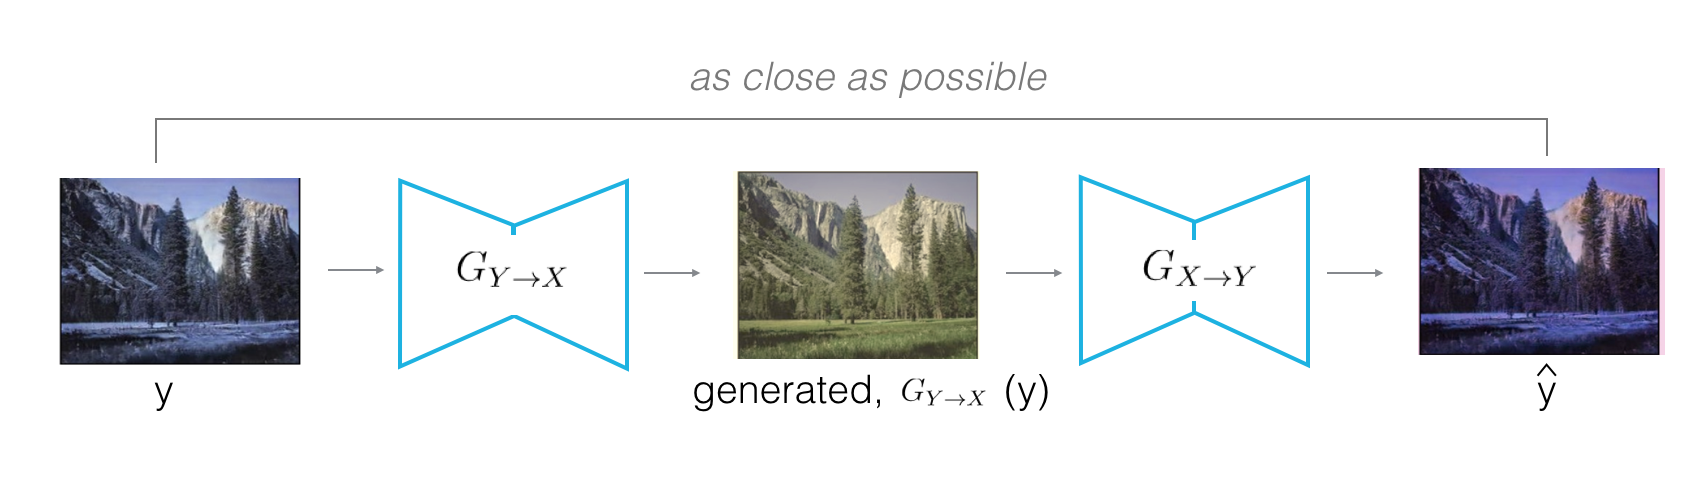
\includegraphics[width=1\linewidth]{img//genAdvNet//image2image/cycle_consistency_ex.png}

\subsubsection{Saving Your Progress}

A CycleGAN repeats its training process, alternating between training
the discriminators and the generators, for a specified number of
training iterations. You've been given code that will save some example
generated images that the CycleGAN has learned to generate after a
certain number of training iterations. Along with looking at the losses,
these example generations should give you an idea of how well your
network has trained.\newline

Below, you may choose to keep all default parameters; your only task is
to calculate the appropriate losses and complete the training cycle.

\begin{lstlisting}[language=Python]
# import save code
from helpers import save_samples, checkpoint
\end{lstlisting}

\begin{lstlisting}[language=Python]
# train the network
n_epochs = 4000 # keep this small when testing if a model first works
print_every=10
    
# keep track of losses over time
losses = []

test_iter_X = iter(test_dataloader_X)
test_iter_Y = iter(test_dataloader_Y)

# Get some fixed data from domains X and Y for sampling. These are images that are held
# constant throughout training, that allow us to inspect the model's performance.
fixed_X = test_iter_X.next()[0]
fixed_Y = test_iter_Y.next()[0]

# batches per epoch
iter_X = iter(dataloader_X)
iter_Y = iter(dataloader_Y)
batches_per_epoch = min(len(iter_X), len(iter_Y))

for epoch in range(1, n_epochs+1):
    # Reset iterators for each epoch
    if epoch % batches_per_epoch == 0:
        iter_X = iter(dataloader_X)
        iter_Y = iter(dataloader_Y)

    images_X, _ = iter_X.next()

    images_Y, _ = iter_Y.next()

    # move images to GPU if available (otherwise stay on CPU)
    device = torch.device("cuda:0" if torch.cuda.is_available() else "cpu")
    images_X = images_X.to(device)
    images_Y = images_Y.to(device)
    G_YtoX = G_YtoX.cuda()

    # ============================================
    #            TRAIN THE DISCRIMINATORS
    # ============================================

    ##   First: D_X, real and fake loss components   ##

    # Train with real images
    d_x_optimizer.zero_grad()

    # 1. Compute the discriminator losses on real images
    out_x = D_X(images_X)
    D_X_real_loss = real_mse_loss(out_x)

    # Train with fake images

    # 2. Generate fake images that look like domain X based on real images in domain Y
    fake_X = G_YtoX(images_Y)

    # 3. Compute the fake loss for D_X
    out_x = D_X(fake_X.detach())
    D_X_fake_loss = fake_mse_loss(out_x)


    # 4. Compute the total loss and perform backprop
    d_x_loss = D_X_real_loss + D_X_fake_loss
    d_x_loss.backward()
    d_x_optimizer.step()


    ##   Second: D_Y, real and fake loss components   ##

    # Train with real images
    d_y_optimizer.zero_grad()

    # 1. Compute the discriminator losses on real images
    out_y = D_Y(images_Y)
    D_Y_real_loss = real_mse_loss(out_y)

    # Train with fake images

    # 2. Generate fake images that look like domain Y based on real images in domain X
    fake_Y = G_XtoY(images_X)

    # 3. Compute the fake loss for D_Y
    out_y = D_Y(fake_Y.detach())
    D_Y_fake_loss = fake_mse_loss(out_y)

    # 4. Compute the total loss and perform backprop
    d_y_loss = D_Y_real_loss + D_Y_fake_loss
    d_y_loss.backward()
    d_y_optimizer.step()


    # =========================================
    #            TRAIN THE GENERATORS
    # =========================================

    ##    First: generate fake X images and reconstructed Y images    ##
    g_optimizer.zero_grad()

    # 1. Generate fake images that look like domain X based on real images in domain Y
    fake_X = G_YtoX(images_Y)

    # 2. Compute the generator loss based on domain X
    out_x = D_X(fake_X)
    g_YtoX_loss = real_mse_loss(out_x)

    # 3. Create a reconstructed y
    # 4. Compute the cycle consistency loss (the reconstruction loss)
    reconstructed_Y = G_XtoY(fake_X)
    reconstructed_y_loss = cycle_consistency_loss(images_Y, reconstructed_Y, lambda_weight=10)


    ##    Second: generate fake Y images and reconstructed X images    ##

    # 1. Generate fake images that look like domain Y based on real images in domain X
    fake_Y = G_XtoY(images_X)

    # 2. Compute the generator loss based on domain Y
    out_y = D_Y(fake_Y)
    g_XtoY_loss = real_mse_loss(out_y)

    # 3. Create a reconstructed x
    # 4. Compute the cycle consistency loss (the reconstruction loss)
    reconstructed_X = G_YtoX(fake_Y)
    reconstructed_x_loss = cycle_consistency_loss(images_X, reconstructed_X, lambda_weight=10)

    # 5. Add up all generator and reconstructed losses and perform backprop
    g_total_loss = g_YtoX_loss + g_XtoY_loss + reconstructed_y_loss + reconstructed_x_loss
    g_total_loss.backward()
    g_optimizer.step()


    # Print the log info
    if epoch % print_every == 0:
        # append real and fake discriminator losses and the generator loss
        losses.append((d_x_loss.item(), d_y_loss.item(), g_total_loss.item()))
        print('Epoch [{:5d}/{:5d}] | d_X_loss: {:6.4f} | d_Y_loss: {:6.4f} | g_total_loss: {:6.4f}'.format(
                epoch, n_epochs, d_x_loss.item(), d_y_loss.item(), g_total_loss.item()))


    sample_every = 100
    # Save the generated samples
    if epoch % sample_every == 0:
        G_YtoX.eval() # set generators to eval mode for sample generation
        G_XtoY.eval()
        save_samples(epoch, fixed_Y, fixed_X, G_YtoX, G_XtoY, batch_size=16)
        G_YtoX.train()
        G_XtoY.train()

# uncomment these lines, if you want to save your model
#         checkpoint_every=1000
#         # Save the model parameters
#         if epoch % checkpoint_every == 0:
#             checkpoint(epoch, G_XtoY, G_YtoX, D_X, D_Y)

\end{lstlisting}

\subsection{Tips on Training and Loss
Patterns}

A lot of experimentation goes into finding the best hyperparameters such
that the generators and discriminators don't overpower each other. It's
often a good starting point to look at existing papers to find what has
worked in previous experiments, I'd recommend this
\href{https://arxiv.org/pdf/1511.06434.pdf}{DCGAN paper} in addition to
the original \href{https://arxiv.org/pdf/1703.10593.pdf}{CycleGAN paper}
to see what worked for them. Then, you can try your own experiments
based off of a good foundation.

\paragraph{Discriminator Losses}

When you display the generator and discriminator losses you should see
that there is always some discriminator loss; recall that we are trying
to design a model that can generate good ``fake'' images. So, the ideal
discriminator will not be able to tell the difference between real and
fake images and, as such, will always have some loss. You should also
see that \(D_X\) and \(D_Y\) are roughly at the same loss levels; if
they are not, this indicates that your training is favoring one type of
discriminator over the and you may need to look at biases in your models
or data.

\paragraph{Generator Loss}

The generator's loss should start significantly higher than the
discriminator losses because it is accounting for the loss of both
generators \emph{and} weighted reconstruction errors. You should see
this loss decrease a lot at the start of training because initial,
generated images are often far-off from being good fakes. After some
time it may level off; this is normal since the generator and
discriminator are both improving as they train. If you see that the loss
is jumping around a lot, over time, you may want to try decreasing your
learning rates or changing your cycle consistency loss to be a little
more/less weighted.

\begin{lstlisting}[language=Python]
fig, ax = plt.subplots(figsize=(12,8))
losses = np.array(losses)
plt.plot(losses.T[0], label='Discriminator, X', alpha=0.5)
plt.plot(losses.T[1], label='Discriminator, Y', alpha=0.5)
plt.plot(losses.T[2], label='Generators', alpha=0.5)
plt.title("Training Losses")
plt.legend()
\end{lstlisting}

\subsection{Evaluate the Result}

As you trained this model, you may have chosen to sample and save the
results of your generated images after a certain number of training
iterations. This gives you a way to see whether or not your Generators
are creating \emph{good} fake images. For example, the image below
depicts real images in the \(Y\) set, and the corresponding generated
images during different points in the training process. You can see that
the generator starts out creating very noisy, fake images, but begins to
converge to better representations as it trains (though, not perfect).

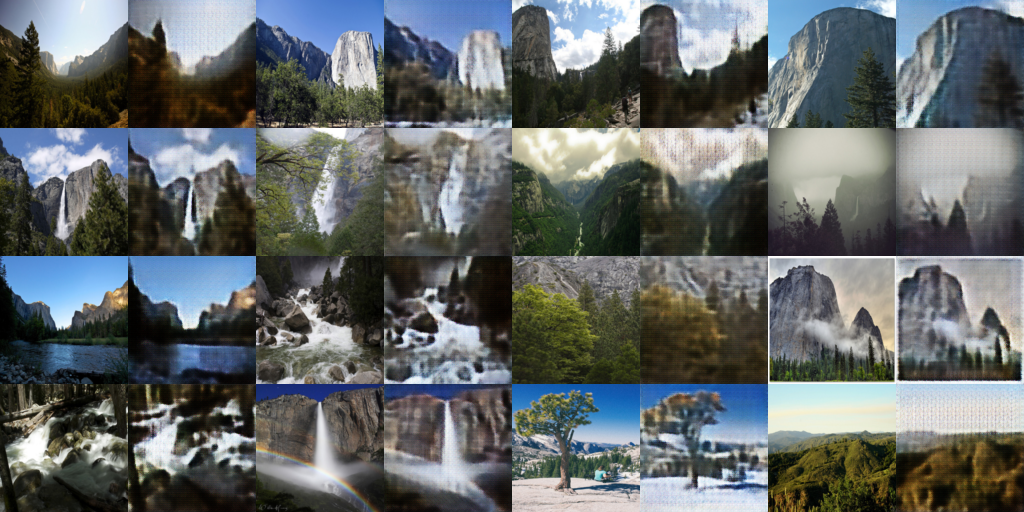
\includegraphics[width=0.5\linewidth]{img//genAdvNet//image2image/sample-004000-summer2winter.png}

Below, you've been given a helper function for displaying generated
samples based on the passed in training iteration.

\begin{lstlisting}[language=Python]
import matplotlib.image as mpimg

# helper visualization code
def view_samples(iteration, sample_dir='samples_cyclegan'):
    
    # samples are named by iteration
    path_XtoY = os.path.join(sample_dir, 'sample-{:06d}-X-Y.png'.format(iteration))
    path_YtoX = os.path.join(sample_dir, 'sample-{:06d}-Y-X.png'.format(iteration))
    
    # read in those samples
    try: 
        x2y = mpimg.imread(path_XtoY)
        y2x = mpimg.imread(path_YtoX)
    except:
        print('Invalid number of iterations.')
    
    fig, (ax1, ax2) = plt.subplots(figsize=(18,20), nrows=2, ncols=1, sharey=True, sharex=True)
    ax1.imshow(x2y)
    ax1.set_title('X to Y')
    ax2.imshow(y2x)
    ax2.set_title('Y to X')
\end{lstlisting}

\begin{lstlisting}[language=Python]
# view samples at iteration 100
view_samples(100, 'samples_cyclegan')
\end{lstlisting}

\begin{lstlisting}[language=Python]
# view samples at iteration 4000
view_samples(4000, 'samples_cyclegan')
\end{lstlisting}

\subsection{Further Challenges and Directions}

\begin{itemize}

\item One shortcoming of this model is that it produces fairly
  low-resolution images; this is an ongoing area of research; you can
  read about a higher-resolution formulation that uses a multi-scale
  generator model, in \href{https://arxiv.org/abs/1711.11585}{this
  paper}.
\item Relatedly, we may want to process these as larger (say 256x256) images
  at first, to take advantage of high-res data.
\item It may help your model to converge faster, if you initialize the
  weights in your network.
\item This model struggles with matching colors exactly. This is because, if
  \(G_{YtoX}\) and \(G_{XtoY}\) may change the tint of an image; the
  cycle consistency loss may not be affected and can still be small. You
  could choose to introduce a new, color-based loss term that compares
  \(G_{YtoX}(y)\) and \(y\), and \(G_{XtoY}(x)\) and \(x\), but then
  this becomes a supervised learning approach.
\item This unsupervised approach also struggles with geometric changes, like
  changing the apparent size of individual object in an image, so it is
  best suited for stylistic transformations.
\item For creating different kinds of models or trying out the Pix2Pix
  Architecture,
  \href{https://github.com/junyanz/pytorch-CycleGAN-and-pix2pix/}{this
  Github repository} which implements CycleGAN \emph{and} Pix2Pix in
  PyTorch is a great resource.
\end{itemize}

\textbf{Once you are satified with your model, you are ancouraged to
test it on a different dataset to see if it can find different types of
mappings}

\subsubsection{Different datasets for download}

You can download a variety of datasets used in the Pix2Pix and CycleGAN
papers, by following instructions in the
\href{https://github.com/junyanz/pytorch-CycleGAN-and-pix2pix/blob/master/README.md}{associated
Github repository}. You'll just need to make sure that the data
directories are named and organized correctly to load in that data.
